% RolloutSecBench - Figure 1: system architecture, attacker capability boundary, and SHA-256 provenance chain.
% Natural width ~17.5 cm (full page width). Box text 7 pt, annotations 6 pt.
% Standalone build:  pdflatex fig1_architecture.tex
% MDPI manuscript (full-width figure):
%   \begin{figure}[H]\begin{adjustwidth}{-\extralength}{0cm}\centering
%     \includegraphics[width=\linewidth]{fig1_architecture.pdf}
%   \end{adjustwidth}\caption{...}\label{fig:architecture}\end{figure}
\documentclass[border=3pt]{standalone}
\usepackage[T1]{fontenc}
\usepackage{helvet}
\renewcommand{\familydefault}{\sfdefault}
\usepackage{amsmath}
\usepackage{tikz}
\usetikzlibrary{arrows.meta,fit,backgrounds,calc}

\definecolor{evid}{RGB}{31,94,160}     % evidence / measurement path
\definecolor{atk}{RGB}{176,38,38}      % attacker capability boundary
\definecolor{lane}{RGB}{245,245,245}
\definecolor{rail}{RGB}{95,95,95}
\newcommand{\sixpt}{\fontsize{6}{7}\selectfont}

\begin{document}
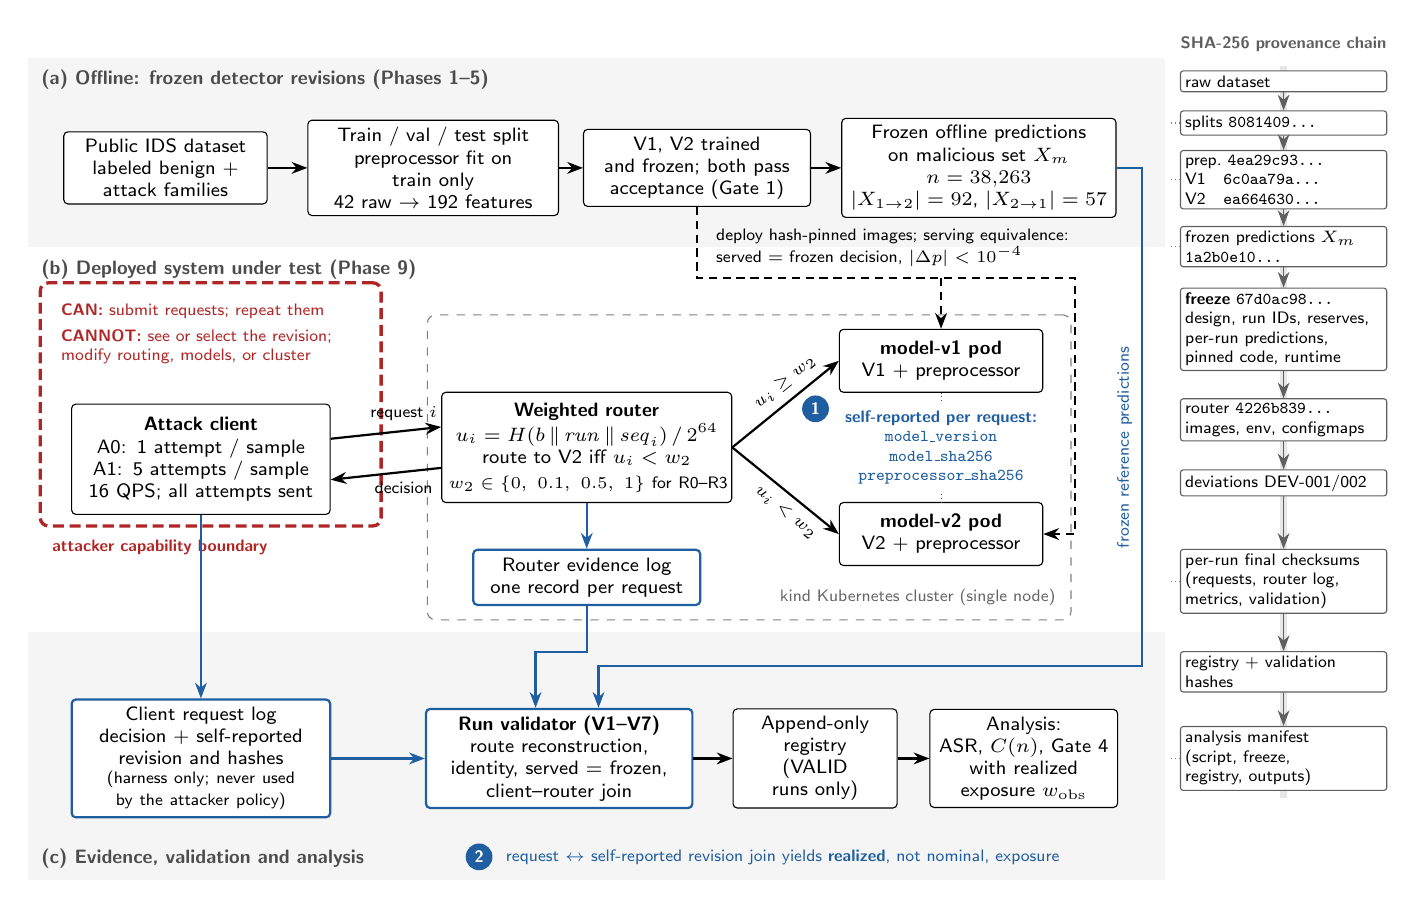
\begin{tikzpicture}[
  font=\scriptsize,
  >={Stealth[length=2mm]},
  box/.style={draw, rounded corners=1.5pt, align=center, fill=white, inner sep=2.6pt, minimum height=8mm},
  ebox/.style={box, draw=evid, thick},
  flow/.style={->, thick},
  eflow/.style={->, thick, evid},
  note/.style={align=center, font=\sixpt},
  badge/.style={circle, fill=evid, text=white, inner sep=0pt, font=\sixpt\bfseries, minimum size=3.4mm},
  hnode/.style={draw=rail, fill=white, rounded corners=1pt, align=left, font=\sixpt, inner sep=1.7pt, text width=25mm},
  lanelab/.style={font=\scriptsize\bfseries, anchor=north west, text=black!70},
]

% ======================================================= lanes
\begin{scope}[on background layer]
  \fill[lane] (-0.2,7.55) rectangle (14.25,9.95);
  \fill[lane] (-0.2,2.65) rectangle (14.25,-0.50);
\end{scope}
\node[lanelab] at (-0.15,9.92) {(a) Offline: frozen detector revisions (Phases 1--5)};
\node[lanelab] at (-0.15,7.50) {(b) Deployed system under test (Phase 9)};
\node[lanelab, anchor=south west] at (-0.15,-0.47) {(c) Evidence, validation and analysis};

% ======================================================= (a) offline pipeline
\node[box, text width=24mm] (data)   at (1.55,8.55) {Public IDS dataset\\labeled benign +\\attack families};
\node[box, text width=30mm] (split)  at (4.95,8.55) {Train / val / test split\\preprocessor fit on\\train only\\42 raw $\rightarrow$ 192 features};
\node[box, text width=27mm] (models) at (8.30,8.55) {V1, V2 trained\\and frozen; both pass\\acceptance (Gate 1)};
\node[box, text width=33mm] (frozen) at (11.88,8.55) {Frozen offline predictions\\on malicious set $X_m$\\\mbox{$n = 38{,}263$}\\\mbox{$|X_{1\rightarrow2}| = 92$,\ $|X_{2\rightarrow1}| = 57$}};
\draw[flow] (data) -- (split);
\draw[flow] (split) -- (models);
\draw[flow] (models) -- (frozen);

% ======================================================= (b) deployed cluster
\node[box, text width=35mm, minimum height=14mm] (router) at (6.90,5.00)
  {\textbf{Weighted router}\\[1pt]
   \mbox{$u_i = H(b \,\|\, \mathit{run} \,\|\, \mathit{seq}_i)\,/\,2^{64}$}\\
   \mbox{route to V2 iff $u_i < w_2$}\\[1pt]
   {\sixpt\mbox{$w_2 \in \{0,\ 0.1,\ 0.5,\ 1\}$ for R0--R3}}};
\node[box, text width=24mm] (p1) at (11.40,6.10) {\textbf{model-v1 pod}\\V1 + preprocessor};
\node[box, text width=24mm] (p2) at (11.40,3.90) {\textbf{model-v2 pod}\\V2 + preprocessor};
\node[ebox, text width=27mm, minimum height=7mm] (rlog) at (6.90,3.35) {Router evidence log\\one record per request};

\draw[flow] (router.east) -- node[pos=0.6, above, sloped, font=\sixpt] {$u_i \ge w_2$} (p1.west);
\draw[flow] (router.east) -- node[pos=0.6, below, sloped, font=\sixpt] {$u_i < w_2$} (p2.west);
\draw[eflow] (router.south) -- (rlog.north);

% badge 1: per-request self-reported identity
\node[note, text=evid, text width=27mm] (selfrep) at (11.40,5.00)
  {\textbf{self-reported per request:}\\\texttt{model\_version}\\\texttt{model\_sha256}\\\texttt{preprocessor\_sha256}};
\node[badge] at ($(selfrep.north west)+(-0.12,-0.10)$) {1};
\draw[evid, thin, densely dotted] (selfrep.north) -- (p1.south);
\draw[evid, thin, densely dotted] (selfrep.south) -- (p2.north);

\node[draw=black!50, dashed, rounded corners=3pt, inner sep=5pt, fit=(router)(p1)(p2)(rlog)(selfrep)] (k8s) {};
\node[font=\sixpt, text=black!60, anchor=south east] at ($(k8s.south east)+(-0.08,0.06)$) {kind Kubernetes cluster (single node)};

% deployment of frozen, hash-pinned artifacts
\draw[flow, densely dashed] (models.south) -- (8.30,7.15) -- (13.10,7.15) -- (13.10,3.90) -- (p2.east);
\draw[flow, densely dashed] (11.40,7.15) -- (p1.north);
\node[note, anchor=south west, align=left] at (8.42,7.17)
  {deploy hash-pinned images; serving equivalence:\\served $=$ frozen decision, $|\Delta p| < 10^{-4}$};

% ======================================================= attacker capability boundary
\node[note, text=atk, anchor=north west, align=left, text width=38mm] (can) at (0.10,6.95)
  {\textbf{CAN:} submit requests; repeat them};
\node[note, text=atk, anchor=north west, align=left, text width=38mm] (cannot) at (0.10,6.62)
  {\textbf{CANNOT:} see or select the revision;\\modify routing, models, or cluster};
\node[box, text width=31mm, minimum height=14mm] (client) at (2.00,4.85)
  {\textbf{Attack client}\\A0: 1 attempt / sample\\A1: 5 attempts / sample\\16 QPS; all attempts sent};
\node[draw=atk, very thick, dash pattern=on 4pt off 2pt, rounded corners=3pt, inner sep=4pt,
      fit=(client)(can)(cannot)] (atkbox) {};
\node[font=\sixpt\bfseries, text=atk, anchor=north west] at ($(atkbox.south west)+(0.05,-0.03)$) {attacker capability boundary};

\draw[flow] ([yshift=2.6mm]client.east) -- node[pos=0.66, above, font=\sixpt] {request $i$} ([yshift=2.6mm]router.west);
\draw[flow, <-] ([yshift=-2.6mm]client.east) -- node[pos=0.66, below, font=\sixpt] {decision} ([yshift=-2.6mm]router.west);

% ======================================================= (c) evidence and analysis
\node[ebox, text width=31mm] (clog)  at (2.00,1.05) {Client request log\\decision + self-reported\\revision and hashes\\{\sixpt(harness only; never used\\by the attacker policy)}};
\node[ebox, text width=32mm] (valid) at (6.55,1.05) {\textbf{Run validator (V1--V7)}\\route reconstruction,\\identity, served $=$ frozen,\\client--router join};
\node[box, text width=19mm] (reg)    at (9.80,1.05) {Append-only\\registry\\(VALID runs only)};
\node[box, text width=22mm] (ana)    at (12.45,1.05) {Analysis:\\ASR, $C(n)$, Gate 4\\with realized\\exposure $w_{\mathrm{obs}}$};

\draw[eflow] (client.south) -- (clog.north);
\draw[eflow] (clog.east) -- (valid.west);
\draw[eflow] (rlog.south) -- (6.90,2.40) -- (6.25,2.40) -- (6.25,1.05 |- valid.north);
\draw[eflow] (frozen.east) -- (13.95,8.55) -- (13.95,2.22) -- (7.05,2.22) -- (7.05,1.05 |- valid.north);
\node[font=\sixpt, text=evid, rotate=90, anchor=south] at (13.95,5.00) {frozen reference predictions};
\draw[flow] (valid) -- (reg);
\draw[flow] (reg) -- (ana);

% badge 2: realized exposure
\node[note, text=evid, anchor=west, align=left] (realized) at (5.75,-0.20)
  {request $\leftrightarrow$ self-reported revision join yields \textbf{realized}, not nominal, exposure};
\node[badge, anchor=east] at ($(realized.west)+(-0.04,0)$) {2};

% ======================================================= hash-chain side rail (Section AJ)
\def\rx{15.75}
\node[font=\sixpt\bfseries, text=rail, align=center] at (\rx,10.12) {SHA-256 provenance chain};
\node[hnode] (h1)  at (\rx,9.65) {raw dataset};
\node[hnode] (h2)  at (\rx,9.12) {splits \texttt{8081409\ldots}};
\node[hnode] (h3)  at (\rx,8.40) {prep.\ \texttt{4ea29c93\ldots}\\V1\ \ \ \texttt{6c0aa79a\ldots}\\V2\ \ \ \texttt{ea664630\ldots}};
\node[hnode] (h4)  at (\rx,7.55) {frozen predictions $X_m$\\\texttt{1a2b0e10\ldots}};
\node[hnode] (h5)  at (\rx,6.50) {\textbf{freeze} \texttt{67d0ac98\ldots}\\design, run IDs, reserves,\\per-run predictions,\\pinned code, runtime};
\node[hnode] (h6)  at (\rx,5.35) {router \texttt{4226b839\ldots}\\images, env, configmaps};
\node[hnode] (h7)  at (\rx,4.55) {deviations DEV-001/002};
\node[hnode] (h8)  at (\rx,3.30) {per-run final checksums\\(requests, router log,\\metrics, validation)};
\node[hnode] (h9)  at (\rx,2.15) {registry + validation\\hashes};
\node[hnode] (h10) at (\rx,1.05) {analysis manifest\\(script, freeze,\\registry, outputs)};
\begin{scope}[on background layer]
  \draw[rail, line width=2.4pt, opacity=0.15] (\rx,9.85) -- (\rx,0.55);
\end{scope}
\foreach \a/\b in {h1/h2,h2/h3,h3/h4,h4/h5,h5/h6,h6/h7,h7/h8,h8/h9,h9/h10}
  \draw[->, rail, thin] (\a.south) -- (\b.north);
\foreach \h/\y in {h2/9.12, h3/8.40, h4/7.55, h8/3.30, h10/1.05}
  \draw[rail!80, densely dotted, thin] (\h.west) -- (14.30,\y);
\end{tikzpicture}
\end{document}
